\chapter{Generalization, Leakage, and Evaluation Discipline}

\begin{learninggoals}
\item Explain generalization as the ability of a result to survive new data rather than only the observed sample.
\item Distinguish underfitting and overfitting as different failure modes of the same training process.
\item Use protected train, validation, and test roles as procedural boundaries rather than as vocabulary words.
\item Recognize common leakage patterns before they invalidate an experiment.
\item Use a baseline ladder and simple sanity checks to judge whether a reported win means anything.
\item Produce a one-page evaluation plan before reporting a serious model claim.
\end{learninggoals}

Chapter 2 answered one judgment question: once a model outputs scores, what predictive behavior should count as good? Chapter 3 answers the next one: when can we trust the evidence for that behavior?

This chapter is therefore about claim protection. A result can look excellent because the model learned a real pattern. It can also look excellent because the split leaked, the baseline was weak, the test set quietly became part of development, or the task changed between semesters. The chapter's job is to keep those possibilities separate.

\begin{problemsolvinglens}
Protect the claim by keeping development, external evidence, and baseline comparison separate. A strong-looking score is not enough if the workflow that produced it made the result too easy to win.
\end{problemsolvinglens}

\begin{thinkingtool}
\textbf{Claim protection.} Before trusting a win, ask what part of the pipeline could have let future information, duplicate cases, excessive tuning, or a weak baseline make the score look better than it really is.
\end{thinkingtool}

\section{Opening Dilemma: The Validation Score Looks Great. Can We Trust It?}

Keep the same course-support setting in view from the first two chapters. Suppose a support team trains several early-warning models on historical course data and one of them produces excellent validation recall and a strong final test score. Before celebrating, the team still has to ask harder questions. Were the preprocessing steps learned only from the training data? Was the test set kept external until the end? Did the model beat a serious baseline or only a convenient straw man? Would the result still look strong next semester?

Those questions are not paperwork added after the model. They are what make the number mean anything.

\section{Can the Result Survive New Data? Generalization and Overfitting}

The training loss tells us how well the model matches data it has already seen. The next judgment question is whether the result survives new examples.

\begin{definition}[Generalization]
Generalization is the ability of a model to maintain good performance on unseen examples drawn from the same underlying problem as the training data.
\end{definition}

Two classic failure modes define the landscape:
\begin{itemize}[leftmargin=*]
\item \emph{Underfitting}: the model is too simple, too restricted, or too poorly trained to capture even the main patterns in the training data.
\item \emph{Overfitting}: the model matches the training data too closely, including noise or accidental details that do not hold for new data.
\end{itemize}

One way to see this is through the \emph{generalization gap}, the difference between training performance and performance on held-out data. A small gap does not guarantee excellence, but a large gap is a warning sign that the model has learned something too specific to the observed sample.

Model capacity, meaning how complex a pattern the model can represent, plays a central role here. A more flexible model can represent more complicated functions. That flexibility is useful when the data contains real structure, but dangerous when the data is limited or noisy. Overfitting is not evidence of intelligence. It is evidence that the experimental setup allowed memorization or unstable pattern matching to masquerade as learning.

\begin{figure}[t]
\centering
\definecolor{c3fitBlue}{RGB}{56,103,170}
\definecolor{c3fitRed}{RGB}{180,40,40}
\resizebox{\linewidth}{!}{%
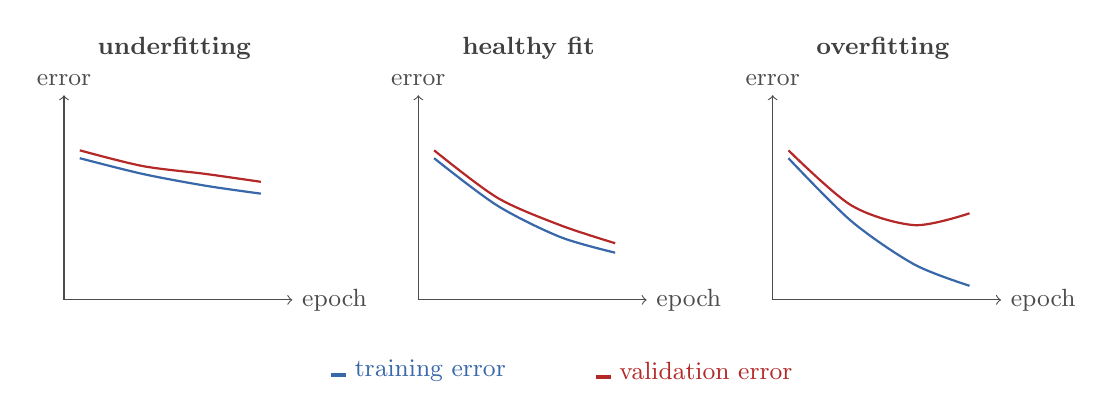
\begin{tikzpicture}[font=\small, x=1cm, y=1cm]
%% Panel 1: underfitting
\begin{scope}[xshift=0cm]
  \node[font=\small\bfseries, black!75] at (1.4,3.2) {underfitting};
  \draw[->,black!70] (0,0) -- (2.9,0) node[right] {epoch};
  \draw[->,black!70] (0,0) -- (0,2.6) node[above] {error};
  \draw[thick,c3fitBlue]  plot[smooth] coordinates {(0.2,1.8)(1.0,1.6)(1.8,1.45)(2.5,1.35)};
  \draw[thick,c3fitRed]   plot[smooth] coordinates {(0.2,1.9)(1.0,1.7)(1.8,1.60)(2.5,1.50)};
\end{scope}
%% Panel 2: healthy fit
\begin{scope}[xshift=4.5cm]
  \node[font=\small\bfseries, black!75] at (1.4,3.2) {healthy fit};
  \draw[->,black!70] (0,0) -- (2.9,0) node[right] {epoch};
  \draw[->,black!70] (0,0) -- (0,2.6) node[above] {error};
  \draw[thick,c3fitBlue]  plot[smooth] coordinates {(0.2,1.8)(1.0,1.2)(1.8,0.80)(2.5,0.60)};
  \draw[thick,c3fitRed]   plot[smooth] coordinates {(0.2,1.9)(1.0,1.3)(1.8,0.95)(2.5,0.72)};
\end{scope}
%% Panel 3: overfitting
\begin{scope}[xshift=9.0cm]
  \node[font=\small\bfseries, black!75] at (1.4,3.2) {overfitting};
  \draw[->,black!70] (0,0) -- (2.9,0) node[right] {epoch};
  \draw[->,black!70] (0,0) -- (0,2.6) node[above] {error};
  \draw[thick,c3fitBlue]  plot[smooth] coordinates {(0.2,1.8)(1.0,1.0)(1.8,0.45)(2.5,0.18)};
  \draw[thick,c3fitRed]   plot[smooth] coordinates {(0.2,1.9)(1.0,1.2)(1.8,0.95)(2.5,1.10)};
\end{scope}
%% Shared legend centered below all three panels
\node[c3fitBlue,  font=\small] at (4.5,-0.9) {\rule{0.6em}{1.5pt}\ training error};
\node[c3fitRed,   font=\small] at (8.0,-0.9) {\rule{0.6em}{1.5pt}\ validation error};
\end{tikzpicture}%
}
\caption{The same training loop can fail in three different ways. Underfitting keeps both errors high. Healthy fitting lowers both while keeping them close. Overfitting continues improving training error while validation error turns upward.}
\label{fig:underfit-healthy-overfit}
\end{figure}

\begin{evidencebox}
Zech et al.\ studied pneumonia detection from chest radiographs across multiple hospital systems and found that generalization changed substantially across institutions; they also analyzed how hospital-specific cues could act as confounders \citep{zech2018}. That is the chapter's lesson in real form: success on familiar held-out data is not the same as robust generalization after deployment.
\end{evidencebox}

\section{Protected Evaluation Workflow}

The next question is procedural rather than mathematical: how do we protect evaluation from development? The answer is the disciplined split between training, validation, and test data.

\begin{itemize}[leftmargin=*]
\item The \emph{training set} is used to fit parameters.
\item The \emph{validation set} is used to choose tuning settings, model structures, thresholds, or stopping points.
\item The \emph{test set} is reserved for the final report after the important decisions are already made.
\end{itemize}

\begin{practicalnote}
The workflow is simple enough to say plainly: split first, fit preprocessing on train only, train candidate models on train, choose among them on validation, and touch the test set once at the end.
\end{practicalnote}

Students often understand those definitions and still run the workflow incorrectly. The key is not only what the sets are called. The key is the order in which they are used.

Here \emph{preprocessing} means data transformations such as scaling, normalization, or feature extraction that are learned from the training data and then applied unchanged to validation and test data.

\begin{figure}[t]
\centering
\definecolor{c3wfRaw}{RGB}{235,242,253}
\definecolor{c3wfRawLine}{RGB}{56,103,170}
\definecolor{c3wfPrep}{RGB}{210,238,220}
\definecolor{c3wfPrepLine}{RGB}{26,112,64}
\definecolor{c3wfTrain}{RGB}{220,233,251}
\definecolor{c3wfTrainLine}{RGB}{56,103,170}
\definecolor{c3wfTune}{RGB}{254,242,214}
\definecolor{c3wfTuneLine}{RGB}{184,92,16}
\definecolor{c3wfTest}{RGB}{237,224,250}
\definecolor{c3wfTestLine}{RGB}{100,50,160}
\resizebox{\linewidth}{!}{%
\begin{tikzpicture}[x=1cm, y=1cm, font=\small,
  raw/.style ={draw=c3wfRawLine,  fill=c3wfRaw,  rounded corners, align=center,
               minimum height=0.9cm, minimum width=2.1cm,
               font=\small\bfseries, text=c3wfRawLine},
  pre/.style ={draw=c3wfPrepLine, fill=c3wfPrep, rounded corners, align=center,
               minimum height=0.9cm, minimum width=2.7cm,
               font=\small\bfseries, text=c3wfPrepLine},
  trn/.style ={draw=c3wfTrainLine,fill=c3wfTrain,rounded corners, align=center,
               minimum height=0.9cm, minimum width=2.3cm,
               font=\small\bfseries, text=c3wfTrainLine},
  tun/.style ={draw=c3wfTuneLine, fill=c3wfTune, rounded corners, align=center,
               minimum height=0.9cm, minimum width=2.1cm,
               font=\small\bfseries, text=c3wfTuneLine},
  tst/.style ={draw=c3wfTestLine, fill=c3wfTest, rounded corners, align=center,
               minimum height=0.9cm, minimum width=2.1cm,
               font=\small\bfseries, text=c3wfTestLine},
  arrow/.style={-Latex, thick, black!55}
]
%% ── Top row ──────────────────────────────────────────────────────────
\node[raw] (raw)   at (1.1,  3.2) {Raw data};
\node[raw] (split) at (3.8,  3.2) {Split first};
\node[pre] (prep)  at (7.2,  3.2) {Fit preprocessing\\on train only};
%% ── Bottom row ───────────────────────────────────────────────────────
\node[trn] (train) at (3.8,  0.9) {Train candidate\\models};
\node[tun] (tune)  at (7.2,  0.9) {Tune on\\validation};
\node[tst] (test)  at (10.3, 0.9) {Report once\\on test};
%% ── Arrows ───────────────────────────────────────────────────────────
\draw[arrow] (raw)   -- (split);
\draw[arrow] (split) -- (prep);
\draw[arrow] (split) -- (train);
\draw[arrow] (prep)  -- (tune);
\draw[arrow] (train) -- (tune);
\draw[arrow] (tune)  -- (test);
%% ── Annotation: sits to the right of the prep→tune arrow ─────────────
\node[anchor=west, align=left, font=\footnotesize, black!55]
  at (7.9, 2.05)
  {apply the same\\transform to\\val and test};
\end{tikzpicture}%
}
\caption{A correct evaluation workflow is procedural, not only conceptual. The split comes before the learned preprocessing, and the test set is touched only after the model-selection decisions are finished.}
\label{fig:evaluation-workflow}
\end{figure}

\begin{thinkingtool}
\textbf{Protected test set.} The test set is for one final report, not for development. Once test results influence model choice, the test set stops being an external check.
\end{thinkingtool}

This logic can be expressed as simple pseudocode:

\begin{codeexample}[caption={A disciplined evaluation workflow}]
train_data, validation_data, test_data = split_data(raw_data)

preprocessor = fit_preprocessor(train_data)
train_ready = preprocessor.transform(train_data)
validation_ready = preprocessor.transform(validation_data)
test_ready = preprocessor.transform(test_data)

model_candidates = train_many_models(train_ready)
chosen_model = select_using_validation(model_candidates, validation_ready)
final_score = evaluate_once(chosen_model, test_ready)
print(final_score)
\end{codeexample}

Cross-validation is a useful extension when data is limited. Instead of relying on one validation split, the training data is partitioned into several folds, meaning several train-validation partitions, and the validation role is rotated across them. Even then, a final untouched test set remains valuable when possible.

\begin{practicalnote}
Chapter 3 establishes minimal experimental discipline for one credible result. Chapter 11 returns to the same logic at larger scale with repeated runs, ablations, slice analysis, and stronger empirical claims.
\end{practicalnote}

\section{How Experiments Lie: Leakage}

Data leakage occurs when information from outside the legitimate training process reaches the model or the experiment design. Leakage is dangerous because it often produces excellent-looking results for the wrong reason.

Common forms of leakage include:
\begin{itemize}[leftmargin=*]
\item normalizing or scaling the full dataset before the train-test split
\item selecting features using all examples before separating the test set
\item using duplicate or near-duplicate examples across training and test data
\item allowing future information into a prediction task that should use only past information
\item tuning repeatedly on the test set until the score looks good
\end{itemize}

Leakage is not a small classroom mistake. Bernett et al.\ present it as a recurring threat to validity in machine learning for biology and argue that guarding against it is central to trustworthy evaluation and reproducibility \citep{bernett2024}. The setting in their paper is biological ML, but the lesson is completely general.

\begin{figure}[t]
\centering
\definecolor{c3lkNeutBg}{RGB}{235,242,253}
\definecolor{c3lkNeutLine}{RGB}{56,103,170}
\definecolor{c3lkWrongBg}{RGB}{254,216,216}
\definecolor{c3lkWrongLine}{RGB}{180,40,40}
\definecolor{c3lkRightBg}{RGB}{210,238,220}
\definecolor{c3lkRightLine}{RGB}{26,112,64}
\resizebox{\linewidth}{!}{%
\begin{tikzpicture}[x=1cm, y=1cm, font=\small,
  neut/.style ={draw=c3lkNeutLine,  fill=c3lkNeutBg,  rounded corners, align=center,
                minimum height=0.85cm, minimum width=1.9cm, font=\small},
  wrong/.style={draw=c3lkWrongLine, fill=c3lkWrongBg, rounded corners, align=center,
                minimum height=0.85cm, minimum width=2.6cm,
                font=\small\bfseries, text=c3lkWrongLine},
  right/.style={draw=c3lkRightLine, fill=c3lkRightBg, rounded corners, align=center,
                minimum height=0.85cm, minimum width=2.3cm,
                font=\small\bfseries, text=c3lkRightLine},
  arrow/.style={-Latex, thick, black!55}
]
%% ── Wrong pipeline ─────────────────────────────────────────────
\node[font=\small\bfseries, c3lkWrongLine] at (0.95, 4.3) {Wrong pipeline};
\node[neut]  (w1) at (0.95, 3.5) {raw data};
\node[wrong] (w2) at (4.0,  3.5) {scale or select\\using all data};
\node[neut]  (w3) at (7.6,  3.5) {split and\\evaluate};
\draw[arrow] (w1) -- (w2);
\draw[arrow] (w2) -- (w3);
%% warning annotation — sits fully below the wrong pipeline row
\node[c3lkWrongLine, font=\small\bfseries] at (4.0, 2.5)
  {test information leaked backward};
\draw[->, thin, c3lkWrongLine] (4.0, 2.75) -- (4.0, 3.07);

%% ── Right pipeline ─────────────────────────────────────────────
\node[font=\small\bfseries, c3lkRightLine] at (0.95, 1.6) {Right pipeline};
\node[neut]  (r1) at (0.95, 0.8) {raw data};
\node[right] (r2) at (3.7,  0.8) {split first};
\node[right] (r3) at (7.3,  0.8) {fit on train,\\apply to val/test};
\draw[arrow] (r1) -- (r2);
\draw[arrow] (r2) -- (r3);
%% ok annotation — sits fully below the right pipeline row
\node[c3lkRightLine, font=\small\bfseries] at (5.5, -0.2)
  {evaluation stays external};
\draw[->, thin, c3lkRightLine] (5.5, 0.05) -- (5.5, 0.37);
\end{tikzpicture}%
}
\caption{Leakage is usually procedural. The wrong pipeline lets information from validation or test examples influence preprocessing or feature design. The right pipeline keeps those steps inside the training boundary.}
\label{fig:leakage-pipelines}
\end{figure}

\begin{codeexample}[caption={Leakage in one line of pseudocode}]
# Wrong: statistics use all examples, including future test cases.
scaled_all = scale(raw_data)
train_data, test_data = split_data(scaled_all)

# Right: split first, then learn the scaling rule from train only.
train_data, test_data = split_data(raw_data)
scaler = fit_scaler(train_data)
train_data = scaler.transform(train_data)
test_data = scaler.transform(test_data)
\end{codeexample}

\begin{warningbox}
Leakage does not merely make a result slightly noisy. It can destroy the meaning of the experiment. A leaked benchmark score is not a weaker scientific claim; it is often no scientific claim at all.
\end{warningbox}

\section{Baseline Ladder and Sanity Checks}

Before trusting a sophisticated model, ask how well simple methods perform. Always predicting the majority class, using a simple weighted linear model, fitting a small decision tree, or even comparing against a random baseline can reveal whether the task is easy, imbalanced, or poorly specified.

\begin{table}[t]
\centering
\small
\setlength{\tabcolsep}{4pt}
\begin{tabular}{p{2.46cm}p{7.78cm}}
\toprule
Baseline rung & What it tells you \\
\midrule
Majority class or constant prediction & Whether the headline score is beating trivial class imbalance or central tendency \\
Simple weighted model & Whether the task already has a strong low-complexity solution \\
Small tree, simple word-count model, or nearest-neighbor copy rule & Whether modest nonlinear structure or simple representation tricks already explain most of the gain \\
Only then a complex model & Whether additional complexity is buying something real rather than hiding weak experimental design \\
\bottomrule
\end{tabular}
\caption{A baseline ladder keeps evaluation honest. If a sophisticated model is not clearly above a simple rung, the experiment is not yet ready for a strong claim.}
\label{tab:baseline-ladder}
\end{table}

Baselines are not only practical convenience. They are part of the philosophy of evidence. They show whether the new method actually improves on something simple, expose hidden issues such as class imbalance or weak labels, and anchor interpretation. A score of $85\%$ may be excellent or trivial depending on the baseline.

The same habit appears in good course design and good benchmark practice. Starter baselines, public datasets, and example solutions do not make the work trivial. They make the claim legible.

\begin{practicalnote}
Two sanity checks should become automatic:
\begin{itemize}[leftmargin=*]
\item \textbf{Shuffled labels.} If labels are randomized and the model still looks strong, the pipeline is broken.
\item \textbf{Split stability.} If validation performance swings wildly under small changes in the train-validation split, the setup may be too fragile for a strong conclusion.
\end{itemize}
\end{practicalnote}

\section{Metric Failure Gallery}

By this point in the chapter, the reader has seen that no single number settles evaluation. It helps to make that lesson explicit through a small gallery of common metric traps.

\begin{table}[t]
\centering
\small
\setlength{\tabcolsep}{4pt}
\begin{tabular}{@{}>{\raggedright\arraybackslash}p{2.13cm}>{\raggedright\arraybackslash}p{2.54cm}>{\raggedright\arraybackslash}p{5.57cm}@{}}
\toprule
Headline metric & Why it looks reassuring & What it can still hide \\
\midrule
High accuracy & Most predictions are correct overall & Class imbalance may make the system useless on the rare class that matters most \\
Strong ROC or ranking score & The model orders cases well in aggregate & The chosen operating point may still produce too many false alarms or too few true positives for the actual review budget \\
Lower loss or better log loss & Average prediction quality improved & The action threshold, calibration in the high-risk region, or severe-error slice may still be unacceptable \\
\bottomrule
\end{tabular}
\caption{A metric can be locally correct and still globally misleading if it does not match the deployment question.}
\label{tab:evaluation-metric-failure-gallery}
\end{table}

\begin{example}[High Accuracy, No Useful Screening]
A screening model evaluated on a heavily imbalanced dataset may report very high accuracy by predicting the majority class almost all the time. The metric is not numerically wrong. It is simply answering the wrong practical question.
\end{example}

\begin{example}[Strong Ranking, Weak Top-of-Queue Policy]
A triage model can achieve a strong ranking score overall and still place too few true urgent cases in the top twenty reviewed items if prevalence is low or the score distribution is compressed near the operational cutoff. In that setting, the aggregate ranking summary is not enough. The top-of-queue behavior is the real test.
\end{example}

\begin{example}[Better Loss, Worse Operational Region]
A probability model may reduce average log loss while becoming slightly worse calibrated exactly in the score range that triggers human escalation. If decisions are made in that region, the lower loss does not automatically imply a better system.
\end{example}

The lesson is not that metrics are untrustworthy. The lesson is that every metric answers a narrower question than students first assume. Good evaluation therefore asks not only ``what is the score?'' but also ``what behavior is this score summarizing, and what important behavior is still outside it?''

\begin{thinkingtool}
\textbf{Metric failure gallery.} Whenever a headline number looks persuasive, name one failure mode it cannot rule out. If no such failure mode comes to mind, the evaluation may still be too shallowly understood.
\end{thinkingtool}

\section{Chapter Artifact: A Minimal Evaluation Plan}

By the end of Chapter 3, the reader should be able to write a short evaluation plan before reporting any result. The goal is not paperwork. The goal is to make the claim explicit enough that weak evidence and procedural mistakes become visible early. This is the point where decision context, threshold as policy, leakage control, and the baseline ladder become one reusable document.

\begin{table}[t]
\centering
\small
\setlength{\tabcolsep}{4pt}
\begin{tabular}{p{3.2cm}p{7.03cm}}
\toprule
Plan field & What must be written down \\
\midrule
Seven-question focus & Questions 1, 5, 6, and 7: what decision matters, what baseline counts, what evidence supports the claim, and how scores become actions \\
Decision context & What real decision or policy the evaluation is meant to support \\
Primary metric & The main quantity that expresses success for that decision \\
Supporting metrics & Additional metrics needed to expose tradeoffs such as imbalance or calibration \\
Threshold or ranking policy & How scores become actions under real capacity or cost constraints \\
Calibration check & How confidence quality will be inspected if probabilities matter downstream \\
Split protocol & How training, validation, and test roles are separated \\
Leakage controls & What preprocessing or feature steps must stay inside the training boundary \\
Baseline ladder & Which simpler baselines the system must beat before a strong claim is made \\
Claim statement & The exact sentence the final result is supposed to justify \\
\bottomrule
\end{tabular}
\caption{If this plan cannot be written, the evaluation claim is usually still underdesigned.}
\label{tab:evaluation-plan}
\end{table}

\begin{thinkingtool}
\textbf{Evaluation plan.} Before reporting a score, write down the decision context, primary and supporting metrics, threshold or ranking policy, calibration check, split protocol, leakage controls, baseline ladder, and final claim sentence.
\end{thinkingtool}

\section{Common Mistakes in Evaluation}

\begin{mistakebox}
\item \textbf{Optimizing the wrong quantity.} A model can improve its training loss and still fail at the deployment metric.
\item \textbf{Letting the test set become a teacher.} Once test results influence model choice, the final score stops being an external check.
\item \textbf{Reporting one number and hiding the tradeoff.} One metric is rarely enough because accuracy, threshold policy, calibration, and rare-case behavior can differ.
\item \textbf{Skipping leakage and baseline checks.} A contaminated pipeline or a weak baseline does not support a strong claim.
\item \textbf{Comparing complex models without a simple baseline.} You still cannot tell whether the task is genuinely hard or the gain is meaningful.
\end{mistakebox}

\section{Looking Ahead}

This chapter made evaluation discipline explicit: generalization, protected evidence, leakage control, baselines, and claim design. The next chapter asks whether a simple linear model can already solve the task once the representation is chosen well.

\begin{chaptersummary}
\item Chapter 3 asks whether the result survives new evidence rather than only the sample already seen during development.
\item Underfitting and overfitting are different ways a training process can fail to generalize.
\item Protected train, validation, and test roles exist to keep evaluation external to model development.
\item Leakage, weak baselines, and test-set reuse are among the most common ways experiments become self-deceptive.
\item A serious empirical claim needs both a defended metric and a defended workflow.
\item The main deliverable of the chapter is a one-page evaluation plan written before a serious model claim is made.
\end{chaptersummary}

\begin{studyquestions}
\item Why is generalization a better judgment question than training loss alone?
\item How does a validation set differ from a test set in purpose?
\item Why must learned preprocessing stay inside the training boundary?
\item Why is a weak baseline a threat to interpretation rather than only to competitiveness?
\item Why can one strong-looking metric still support a weak claim?
\item Why is an evaluation plan more than paperwork?
\end{studyquestions}

\begin{exercises}
\item Design a train-validation-test workflow for a small tabular dataset. State clearly which choices may use the validation set and which choices must not use the test set.
\item A researcher scales all input features using the mean and variance of the entire dataset before creating train and test splits. Explain why this is leakage.
\item Give one example of a weak baseline and one example of a serious baseline for the same task. Explain what each one would and would not tell you.
\item Propose two sanity checks for a model-development workflow in a domain of your choice, and explain what failure on each check would mean.
\item Use a public task such as sports-shot prediction or news topic classification and state one sensible primary metric, one possible secondary metric, and one failure mode the headline metric cannot rule out.
\item Write a one-page evaluation plan using Table~\ref{tab:evaluation-plan} for either spam filtering, course support, or another application of your choice. If you are carrying one case through the book, write this for the same case as your framing memo and metric worksheet so the three documents can be read together.
\end{exercises}

\begin{challengeexercises}
\item A team tunes ten different model families by checking their performance on the test set and reports the best one. Explain precisely why this invalidates the final claim even if the reported score is numerically correct for that one run.
\item A pipeline beats a strong baseline by a small margin, but the shuffled-label check still reports high performance. Diagnose what kinds of bug or contamination could create that result.
\item A course-support team trains on one semester and evaluates on a random split from the same semester. Explain why that may still exaggerate generalization and propose a better split protocol.
\item Write the strongest honest claim for a model that wins on the main metric, loses on a critical slice, and was compared under unequal tuning effort.
\end{challengeexercises}
